\section*{Tutorial Import Table}
\begin{enumerate}
	
	\item Klik SQL Workshop lalu pilih Utulities dan Data Workshop, ikuti seperti yang ada digambar  
	\begin{figure} [!htbp]
	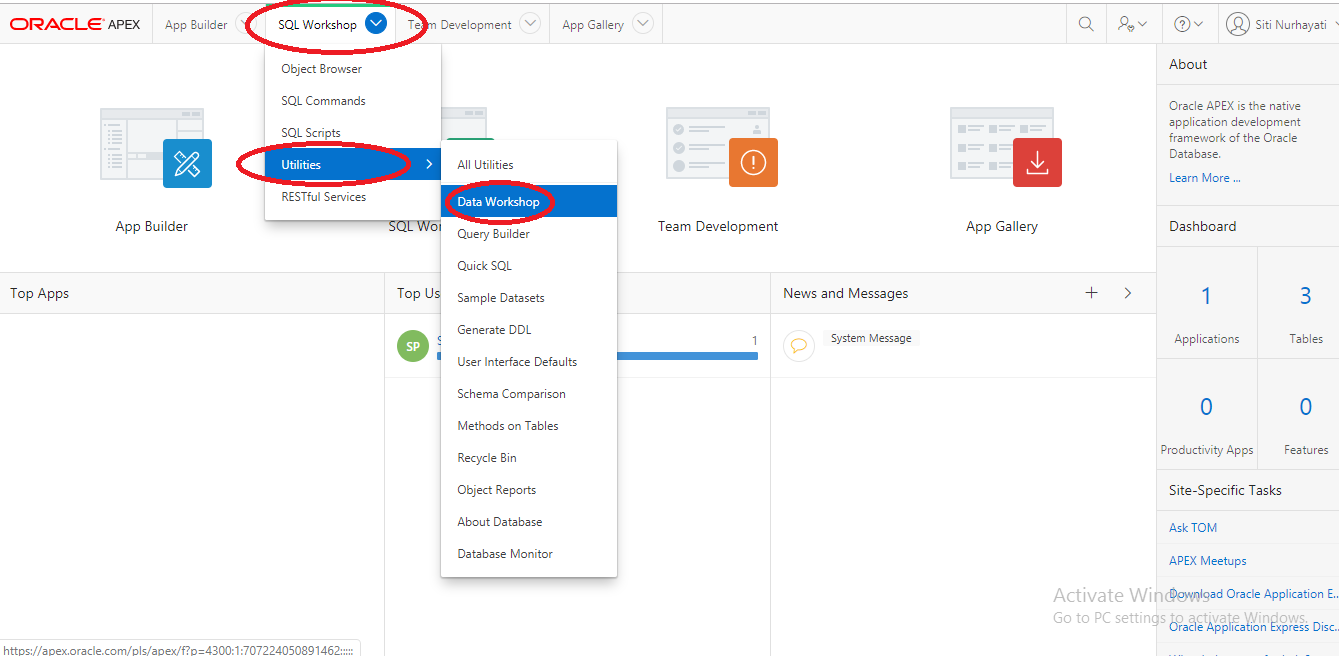
\includegraphics[scale=0.2]{Apex/12.png}
	\centering
	\end{figure}

	\item Siapkan file yang akan di import dan Klik "Load Data" seperti yang ada digambar   
	\begin{figure} [!htbp]
	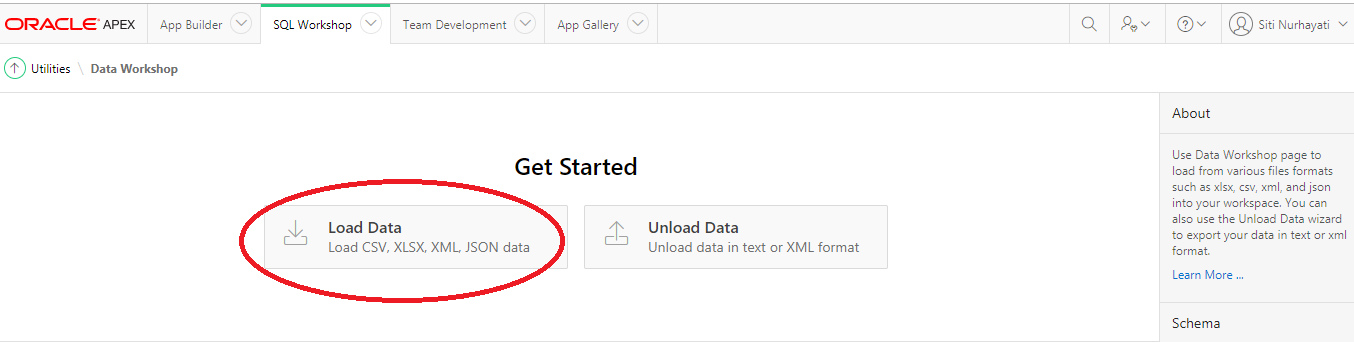
\includegraphics[scale=0.2]{Apex/13.png}
	\centering
	\end{figure}
	
	\item Pilih semua file yang akan di import secara satu-persatu 
	\begin{figure} [!htbp]
	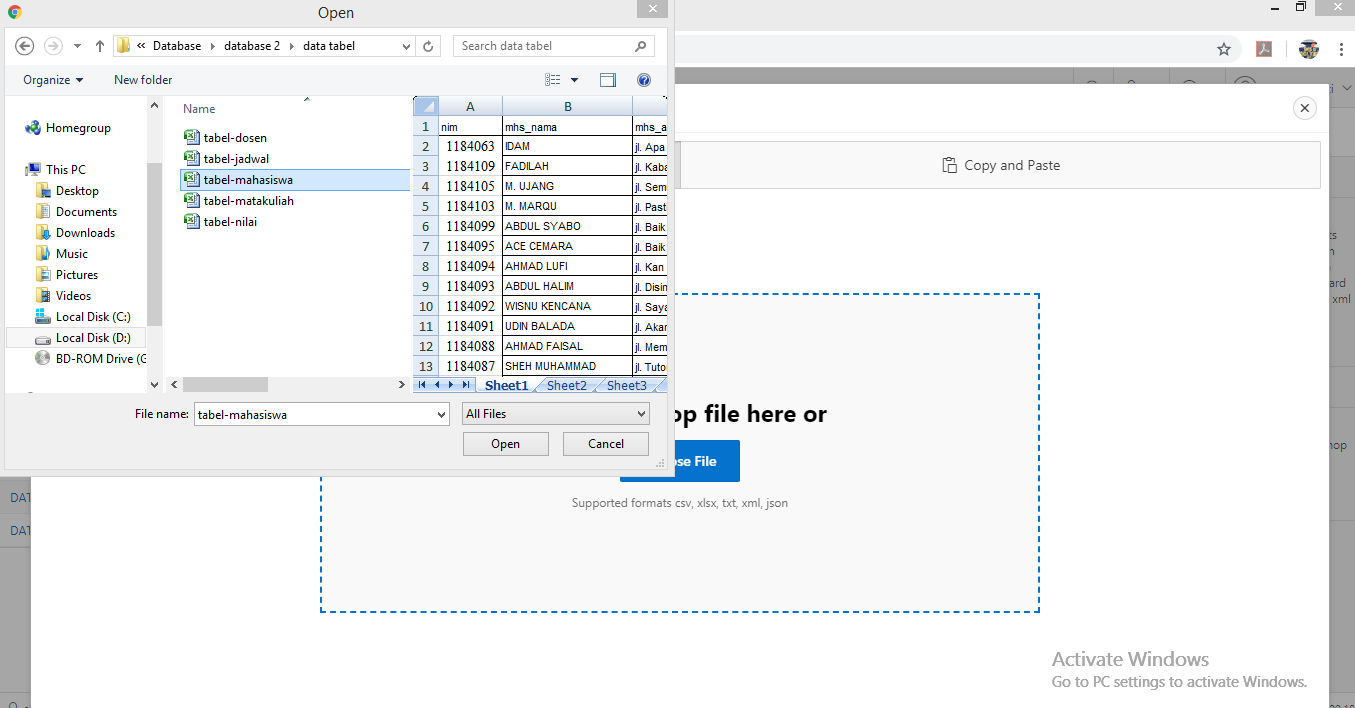
\includegraphics[scale=0.2]{Apex/14.png}
	\centering
	\end{figure}
	
	\item Isi Nama tabel dengan yang kita inginkan lalu klik eror table maka ia akan otomatis terisi dan klik configure 
	\begin{figure} [!htbp]
	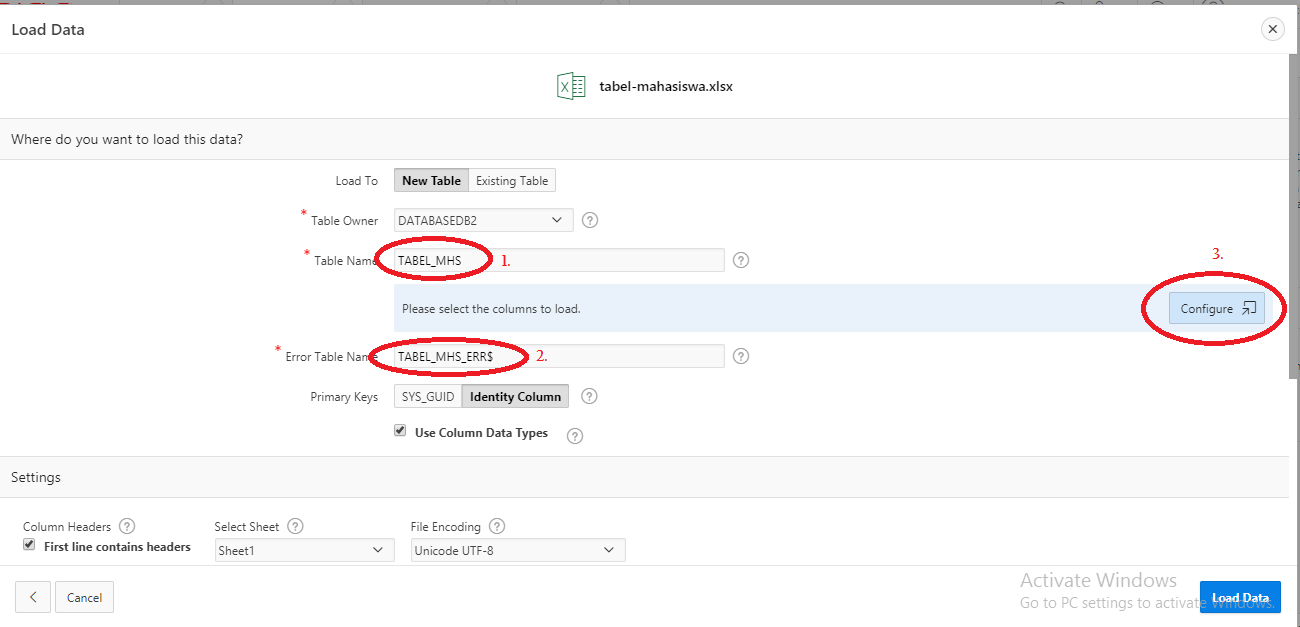
\includegraphics[scale=0.2]{Apex/15.png}
	\centering
	\end{figure}
	
	\item Lalu klik "Save Change" karena tidak ada data yang akan dirubah 
	\begin{figure} [!htbp]
	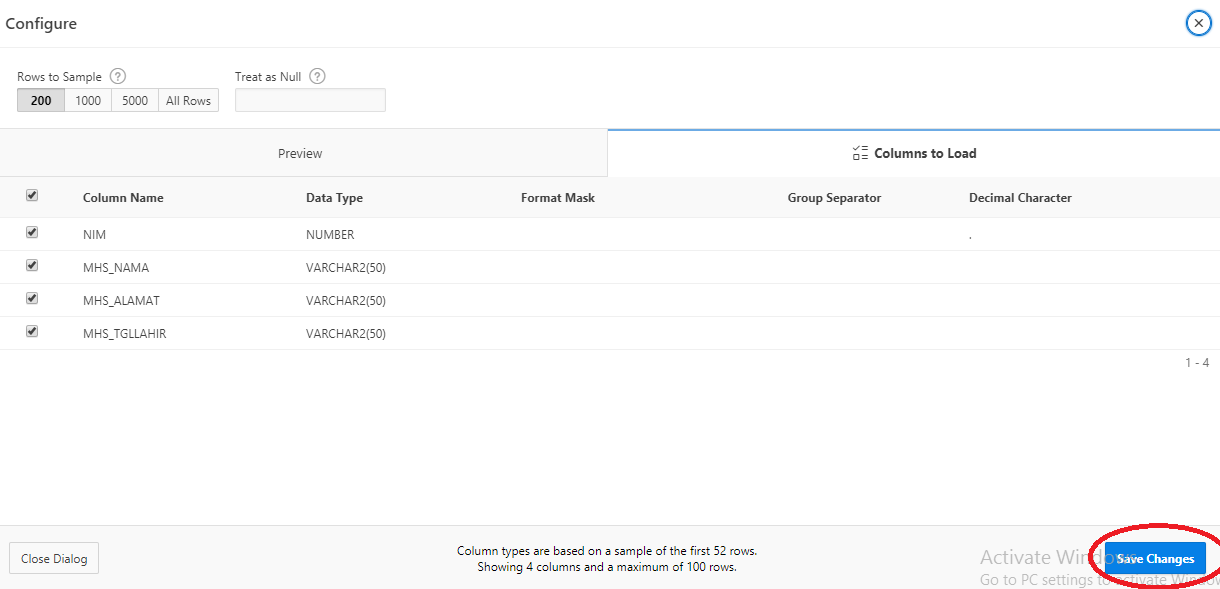
\includegraphics[scale=0.2]{Apex/17a.png}
	\centering
	\end{figure}
	
	\item Klik close terlebih dahulu 
	\begin{figure} [!htbp]
	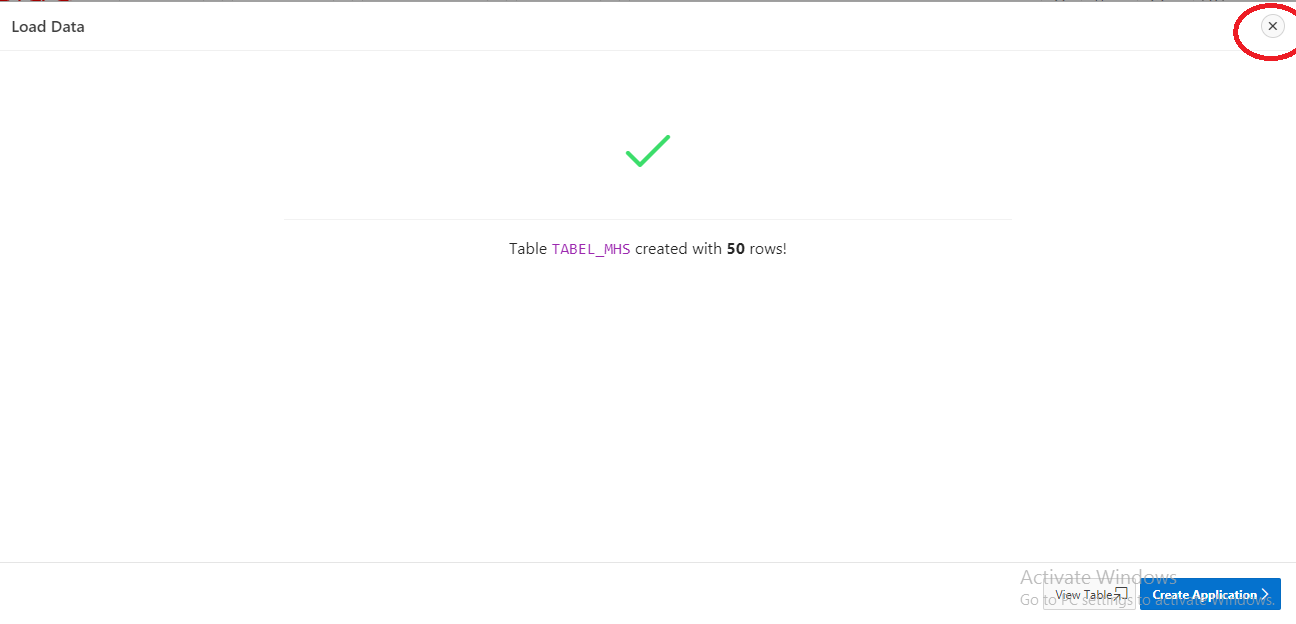
\includegraphics[scale=0.2]{Apex/17.png}
	\centering
	\end{figure}
	
	\item lakukan langkah-langkah seperti diatas pada tabel dosen,jadwal,mata kuliah, dan nilai juga
	
	
\end{enumerate}
